% this is a test
\documentclass[12pt]{article}
\usepackage[margin=1in]{geometry}
\usepackage{fixltx2e}
\usepackage[utf8]{inputenc}

 \usepackage{wrapfig}%   wrap figures/tables in text (i.e., Di Vinci style)
 \usepackage{amsmath}
 \usepackage{amssymb}
 \usepackage{tabu}
 \usepackage{tikz}
 \usetikzlibrary{arrows, shapes, automata,positioning,decorations.pathreplacing}
 \newcommand{\textunderscript}[1]{$_{\text{#1}}$}
 \graphicspath{ {images/} }
\usepackage{titlesec}
\newcommand{\sectionbreak}{\clearpage}

\usepackage{setspace}
\doublespacing

\author{Caris Moses}
\title{Multi-Agent UAV Planning Using BHPN}
\date{\vspace{-5ex}}
%\date{}  % Toggle commenting to test

\begin{document}

\maketitle

\tableofcontents

\section{Introduction}

Planning long duration missions for unmanned aerial vehicles (UAVs) in dynamic environments has proven to be a very challenging problem. Tactical UAVs must be able to reason about how to best accomplish mission objectives in the face of evolving mission conditions. Examples of UAV missions consist of executing multiple tasks such as: locating, identifying, and prosecuting targets; avoiding dynamic (i.e. pop-up) threats; geometric path planning with kinematic and dynamic constraints; and/or acting as a communication relay \cite{cambone2005unmanned}. The resulting planning problem is then one over a large and stochastic state space due to the size of the mission environment and the number of objects within that environment. The world state is also only partially observable due to sensor noise, and requires us to plan in the belief space, which is a probability distribution over all possible states. Some \textit{a priori} contextual knowledge, like target and threat locations, is available via satellite imagery based maps. But it is possible this will be ``old" data by execution time. This makes classic approaches to \textit{a priori} task, or symbolic, planning a poor choice of tool. In addition, task planners traditionally do not have methods for handling geometric planning problems as they focus on high level tasks. However, modern belief space geometric planning tools become intractable for large state spaces, such as ours.

Simply developing a set of ordered tasks, as those produced by purely symbolic approaches like hierarchical task networks~\cite{erol1994htn}, provides a means of generating high-level plans in domains where many different types of actions are possible, as in our domain. But, those methods do not take into account the geometric constraints that may arise while trying to perform a mission task (eg. fly a path from point A to point B subject to our knowledge regarding potential threats in the world). Unstructured and partially observable mission environments with unexpected events create the need for a tactical UAV to reason in both the domain geometry as well as task space. For example, if a UAV is tasked with locating a target, it must ensure that there are no threats preventing the completion of this task and monitor this condition throughout the flight. If a threat does pop-up, it must be determined if its location endangers the mission with some probability. If it does, then the threat must be avoided or additional actions must be planned to neutralize the danger with some certainty. All of these potential responses, or additional actions, require motion planning, thus requiring both probabilistic symbolic and geometric reasoning. 

Geometric planning quickly becomes intractable in partially observable domains, or belief spaces\cite{miller2009pomdp, bourgault2003coordinated}, with long planning horizons. However, recent tools in the domain of robotic manipulation have approached this problem by combining symbolic and geometric planning paradigms \cite{kaelbling2010hierarchical, cambon2009hybrid, wolfe2010combined}. One in particular, Hierarchical Planning-in-the-Now in belief space~\cite{kaelbling2012integrated} (BHPN) is a hierarchical planning technique that tightly couples geometric motion planning in belief spaces with symbolic task planning, providing a method for turning large-scale intractable belief space problems into smaller tractable ones. Another facet of this technique is that it is ``aggressively hierarchical", whereby detailed planning is delayed until it is required, hence the moniker ``in the now". It achieves this by adopting ``levels" of task precondition priority~\cite{sacerdoti1974planning}. Thus abstract plans can be constructed initially (eg. look for target, then fly back to base), while more detailed portions of the plan can be constructed \textit{in situ} as more of the mission environment is considered. BHPN also enables functionality to plan for observations that will improve belief space certainty. The trade-off of using this method as compared to more traditional purely symbolic planning or belief space planning methods is that the resulting plans are not optimal with no bounds on sub-optimality. The plans are simply feasible in that the goal objectives are satisfied in the face of a large state space and unknown environment, which is beneficial given this class of problems. 

In addition to all of the complexities associated with UAV mission planning discussed above, it is also common for multiple UAVs to work as a team to accomplish a mission objective. This is due to the fact that some vehicles may have certain sensor capabilities that others lack. Or it could also simply be to spread out and achieve sufficient coverage of an environment. In general, centralized multi-agent planning (MAP) is exponential in the number of agents. Therefore, we took a decentralized planning approach to enabling UAV teaming. BHPN provides a good method of implementing this loosely-coupled MAP effort. The BHPN framework of using preconditions to bind objects in the physical world to executable actions is used to select the correct UAV to execute an action based on its sensor capabilities. As with single-agent planning, in MAP when a UAV is receiving help it continues to develop future plans assuming that the help it requires will be successful, and replanning if it is not.

This research focuses on reapplying the BHPN framework to plan and execute UAV missions in unstructured domains. I will show this by first outlining related work in the field of task, motion, and integrated planning. Then explain how the BHPN framework was changed to support both the abilities of a tactical UAV and the mission environment it is required to plan in. Then I will explain how this framework was extended to the problem of MAP. An analysis of the BHPN algorithm is proposed as well as a realistic mission simulation and some sample mission scenarios.

\section{Background}

\subsection{Related Work}

Integrated task and motion planning requires a method of developing feasible actions which manipulate the world at a high level, as well as a method of planning efficient motions on a low level. In this related work section we will address task planning methods in Section \ref{task planning}, and motion planning methods in Section \ref{motion planning}. We will also look at methods other than BHPN which handle the integration of the two in Section \ref{integrated planning}. A more detailed discussion about belief space planning, specifically partially observable Markov decision processes (POMDPs) is given in section \ref{POMDP}. Finally, other methods of MAP are given in section \ref{MAP}.

\subsubsection{Task Planners} \label{task planning}

Task planning consists of searching for an action sequence which will transform the current world state into a goal state. STRIPS~\cite{fikes1972strips} (Stanford Research Institute Problem Solver) was the first widely used task planner. STRIPS employs a method of classical planning where the action sequence is found using backward-chaining state space search. Heuristics can be used to speed up this process such as partial-order planning~\cite{barrett1994partial} which loosens restrictions on the order in which actions must be executed. Hierarchal methods, such as  HTN~\cite{erol1994htn} (hierarchical task networks), provide significant speedups when compared to classical planning approaches~\cite{bylander1994computational}. HTN uses a combination of primitive tasks, compound tasks, and goal tasks to reduce the problem solving effort. A shortcoming of all aforementioned task planners is that they do not provide a means for executing an action. For example, if a task is to place block 1 on top of block 2, it will not provide a trajectory for the robot arm to follow as it places the block, or a grasp with which to hold the block. For that we require a low-level motion planner.

\subsubsection{Motion Planners} \label{motion planning}

The field of motion planning is rich with proposed methods, particularly where they apply to uncertain domains. In the UAV domain the motion planning problem is often to localize and track targets~\cite{miller2009pomdp}. One method is to solve a partially observable Markov decision process (POMDP)~\cite{ponzoni2012pomdp, chanel2013multi}. However, solving a POMDP is generally computationally intractable~\cite{hauskrecht2000value}. A common approximation is to use receding horizon control as opposed to solving for an infinite time horizon~\cite{murphy2000survey}. Another approximation is nominal belief optimization which uses a finite-dimensional representation of the belief space and provides a simplification to the objective function which is specific to the tracking problem~\cite{miller2009pomdp}.

Another method of motion planning in belief space for UAVs is to minimize the mean time to detection, or the expected time to find a target~\cite{bourgault2003coordinated, geyer2008active}. The cost function is dependent on action sequences, and the solution is quasi-optimal. As with POMDPs, the solution approaches the optimal solution as more actions are considered when looking ahead. Entropy, or the uncertainty associated with a target's location, can also guide a UAV's search~\cite{carpin2011searching}.

Methods for optimal motion planning are intractable largely due to the long time horizon. BHPN breaks the motion planning problem into multiple motion planning problems. By employing this method, we can utilize strong path planning algorithms for successive short duration flights, or we ``plan in the now".

\subsubsection{Integrated Task and Motion Planning} \label{integrated planning}

Task planning gives a practical method for describing and planning in an environment at a high level. It is well suited for static environments with simple actions where little geometric knowledge is required. These planners require \textit{a priori} knowledge of the domain which become obsolete in the face of a rapidly changing environment (on both a logical and geometric level). On the other hand, purely geometric planners are effective at providing a means of motion through a potentially dynamic and stochastic world. However, geometric planning techniques quickly become intractable for long duration missions with rapidly evolving environments. They also have no method for interpreting possible actions other than those pertaining to motion. For these reasons, previous work has sought to combine task and motion planning. In these domains there are many high-level tasks that need to be considered and low-level motions (eg. grasps, arm trajectories, or paths) that need to be planned for.

Most recent work in the field of integrated task and motion planning is applied to mobile manipulation in unstructured environments. Some tasks which have been experimented with include cooking a meal~\cite{beetz2011robotic}, pushing buttons to dial a number~\cite{choi2009combining}, and performing other household tasks~\cite{kaelbling2010hierarchical}. The key to integrated planning is to develop an intelligent connection between logical descriptors and the continuous geometry of the real world. One method plans in the configuration space and initially assumes all motions are valid, then replans closer to execution time to ensure that the assumption still holds~\cite{cambon2009hybrid}. Another method speeds up the motion planning process by caching previously calculated motions and using them in future planning problems~\cite{wolfe2010combined}. Guitton and Fargus give an approach for translating geometric constraints into mathematical penalty functions and uses non-linear programming to solve them in the context of HTN planning~\cite{guitton2009taking}. Lastly, Hauser proposes a probabilistic tree-of-roadmaps planner which samples the task and motion space to develop feasible plans~\cite{hauser2010task}.

\subsubsection{POMDPs} \label{POMDP}

In domains where the world state is only partially observable and actions are non-deterministic, a common method of choosing optimal actions is by solving a POMDP. However, solving a POMDP for large state spaces is intractable as it suffers from both the ``curse of dimensionality" and the ``curse of history." Since the state is only partially observable, it is represented as a probability distribution over all possible states, referred to as a belief state. The ``curse of dimensionality" is due to the fact that the size of the belief space grows exponentially with the size of the state space. A history is the set of all actions and observations taken up to the current time step. The ``curse of history" is due to the fact that the number of these action-observation pairs used when solving for the optimal solution to a POMDP grows exponentially with the planning time horizon. To solve a finite-horizon POMDP is PSPACE-complete, and to solve for an infinite-horizon POMDP it is undecidable~\cite{ross_online_2008}. 

The optimal value iteration algorithm is a dynamic programming method used to solve for the optimal policy of a POMDP. A policy acts as a system's controller, where given a state in observable domains, or a belief in partially observable domains, and an observation, it can determine the next action. Calculating the optimal policy to a POMDP can be done off-line, or before execution. Therefore, when a system begins executing the policy, it can do so with little effort since all optimal values are already known. However, as mentioned above, this can be computationally expensive due to the size of the state space and time horizon. Therefore, approximation methods have been applied to POMDPs to enable online planning. Online planning works by interleaving planning and execution. The planning phase consists of generating a belief tree which represents all possible actions, observations, and successor belief states to some depth $D$. Values are generated for each node using approximations of the value function, and near optimal actions are selected based off of these values. Generally, the belief tree is thrown away after each action is executed, and calculated again after an observation has been made. While this method provides a more feasible way to select actions in partially observable domains, it can still be computationally expensive~\cite{ross_online_2008}. Below are two methods of approximating online planning algorithms.

A POMCP works by representing the belief nodes in the belief tree as samples, or states, of the belief probability distribution. $N$ samples are taken from the initial belief, and $m$ simulations are run before selecting the next near-optimal action. A generative model, $g$, of the POMDP is required, where $(s', o, r) = g(s, a)$. Given a state and an action, it returns a successor state, an observation, and an immediate a reward. Each node in the belief tree stores an average expected value from all simulations, as well as a visitation count. At the beginning of the simulation a starting state is selected from the initial belief state samples, and an action is selected based on the action nodes' expected values as well as their visitation counts (to encourage exploring new areas of the tree). The generative model is called with this sampled state and selected action and the immediate reward is returned. To calculate the total expected reward of this successor state, the delayed reward, in addition to the immediate reward, is needed. The delayed reward is the reward received from the successor state to the goal state. If the successor state exists within the belief tree, then the simulation continues recursively. If a successor node is not within the tree, then a random rollout policy is used to calculate the delayed reward. Once this simulation has been completed $m$ times, an action node from the root belief node with the highest value is selected. Since the belief nodes are represented as particles, a particle filter is used to perform the belief space update~\cite{silver_monte-carlo_2010}.

This algorithm deals with the curse of dimensionality by representing beliefs in the belief tree as a sample of states, or particles, from the belief state. It handles the curse of history by sampling histories using the generative model. By using this model, the complexity of the algorithm depends on the complexity of the generative model, and not the underlying POMDP~\cite{silver_monte-carlo_2010}.

DESPOT also represents a belief state as a sample of particles from the belief state distribution. The POMCP algorithm can suffer from overfitting. To compensate for this, a DESPOT is a sparse belief tree, generated by $K$ sampled scenarios. The resulting tree contains all possible actions, but only observations from the sampled scenarios. This greatly reduces the complexity of the search tree, while still maintaining a good approximation of the entire belief tree. Once the tree is generated, dynamic programming is used to calculate the optimal policy within the tree. Heuristics and branch-and-bound are also used during the tree construction to ensure that only promising branches are included, and that overfitting does not occur~\cite{somani_despot:_2013}.

\subsubsection{Multi-Agent Planning} \label{MAP}

\subsection{BHPN Description} \label{bhpn description}

The following BHPN description is based on work by Kaelbling and Lozano-P{\'e}rez~\cite{kaelbling2012integrated}. Integrated task and motion planning requires a means of connecting the high-level task space with the low-level geometric space. BHPN achieves this through the use of fluent, or logical descriptors. Fluents can contain information about the continuous geometric space, or belief space, as well as discrete attributes about the environment. They give information such as the certainty that an object is in a given location, or even the contents of a location. The initial belief state, as well as the goal state, are described in terms of fluents. Operators, or tasks, manipulate these fluents in order to achieve the goal state. Operators consist of a primitive action, preconditions, and an effect. A primitive action is the component of an operator which is executed in the world, and all preconditions must be satisfied in order for this to take place. The effect is a fluent which should become True after the primitive action is executed. Another critical component of operators are generator functions, which are used to tie geometric constraints (eg. ensure that there is a clear path) in with task-oriented planning. 

BHPN develops plans through goal regression, or pre-image backchaining. Plans consist of an ordered set of (operator, pre-image) tuples. Pre-images are sets of fluents such that for an operator to be executed, its pre-image must be satisfied in the current world state. When planning hierarchically, many plans are developed, as opposed to flat planning where only one plan is generated. First, an initial abstract plan is created, then the first operator of this plan is expanded into another, more concrete, plan. This process is called plan refinement~\cite{bacchus1994downward}, and it effectively adds additional operators between the ones already in place in the higher level abstract plan. The refining process can be thought of as a tree generation in a depth-first manner (see Figure~\ref{hpn tree}). To determine the set of preconditions necessary to consider when developing a plan, preconditions are assigned abstraction levels. These levels indicate when in the planning process certain preconditions will be considered. For example, the first abstract plan is generated by only considering preconditions at the 0th level. Planning will not continue if there is no means of satisfying a precondition. Therefore, when assigning preconditions levels, it is imperative to put the most critical preconditions first~\cite{sacerdoti1974planning} as well as the preconditions which are the most difficult to satisfy. As the tree is built, eventually an operator will have all of its preconditions satisfied, at which point the primitive is executed. It is this functionality which allows us to ``plan in the now", or perform ``interleaved" planning and execution. When planning, contingency plans are not generated. Plans are assumed to have the expected result on the belief state. This is a very loose assumption, particularly in nondeterministic and dynamic domains where the state is rapidly changing. However a major attribute of BHPN is observing the belief state after a primitive is executed and replanning if an action did not have the expected result. As future plans are simply abstrac onest, not a significant amount of planning effort is lost as replanning occurs.

\subsubsection{Components}

Pre-mission, a set of fluents must be initialized based on the UAV's current knowledge. In general, fluents can be characterized in this way: the \textit{threat} location is \textit{region 1} with certainty \textit{0.5}, or even like this: \textit{region 2} is occupied by a target with certainty \textit{0.8}. The flexibility available when initializing the belief state enables us to incorporate varying degrees of knowledge in many different ways. Concrete examples of fluents will be given in Section \ref{domain operators}. Operators are also user-defined in terms of domain knowledge. Figure~\ref{example operator} gives an example of an operator.

\begin{figure}
\textbf{Operator}: Fly(UAV, start, dest, path, $p$)\\
\textbf{Preconditions}: \\
\indent 0: the UAV is located at the start location with probability $flyRegress(p)$\\
\indent 1: the path is clear with probability $\epsilon$\\
\textbf{Generators}: path = $generatePath$(start, dest)\\
\textbf{Effect}: the UAV is located at the dest location with probability $p$\\
\textbf{Primitive Action}: Fly from the start to the dest location
\label{example operator}
\caption{Example of an operator in the UAV domain.}
\end{figure}

As you can see, the preconditions and effect are fluents. In belief space, fluents are in terms of probabilities since states are only partially observable. An example of a goal would be ``the UAV is located at \textit{region 1} with $0.95$ certainty". Planning uses goal regressio. In order to achieve the goal, we must determine the necessary pre-image. This is where regression functions, such as $flyRegress(p)$ above, come into play. We need to calculate the necessary probability currently in the world in order to successfully Fly the UAV from its start location to \textit{region 1}. The regression function is derived from the underlying transition model of the UAV. If the UAV's actions are highly nondeterministic, then we will need a higher initial certainty before executing the Fly action. But, if our actions are nearly deterministic, then we can easily ensure that after the Fly task is executed, we are certain (greater than 0.95) that the UAV will be located in \textit{region 1}. Regression functions are also important when an operator involves observations, which we will see in Section \ref{uav domain observation}. In this case the regression functions are derived from the underlying UAV observation model.

Another important component of operators are generator functions. These can be used to incorporate geometric constraints. In Figure~\ref{example operator} a generator is used to find a path between the start and dest locations. Then, this path becomes part of a precondition such that it must be clear with $\epsilon$ (user-defined) certainty. Once these two preconditions are satisfied, the UAV will attempt to fly from start to dest.

The final component of the BHPN process is the belief space update. When a primitive action is executed, the UAV must update its belief state based on its own motion or observations it has gathered. This step depends on how the belief space is represented. Methods such as Kalman filtering for Gaussian processes and Bayes filtering for non-Gaussian processes may be implemented.

\subsubsection{Algorithm} \label{bhpn algorithm}

Hierarchical planning is able to improve planning efficiency through the use of abstraction. By giving preconditions abstraction levels, we are actually turning one operator into many operators. For example, the Fly operator is actually a Fly0 operator (only precondition 0 is considered), a Fly1 operator (both preconditions are considered), and a Fly primitive action (where all preconditions are considered). Figure~\ref{hpn tree} shows the planning problem represented as a tree. It is constructed in a depth first manner. The nodes are abstract operators or primitive actions. Plans of  length $k$ are recursively generated, each time planning for an operator at its next abstraction level. The highlighted nodes represent the same operator at different abstraction levels. When the left-most node in the tree is a primitive action, it is immediately executed. Then, planning proceeds until all of the leaf nodes of the tree are primitive actions which have been executed. Each operator is associated with a pre-image (not shown in Fig.~\ref{hpn tree}). Pre-images are sets of fluents which represent what the belief state must look like in order to execute the operator with all of its preconditions met.

\begin{wrapfigure}{R}{0.95\linewidth}

\resizebox{16cm}{!}{
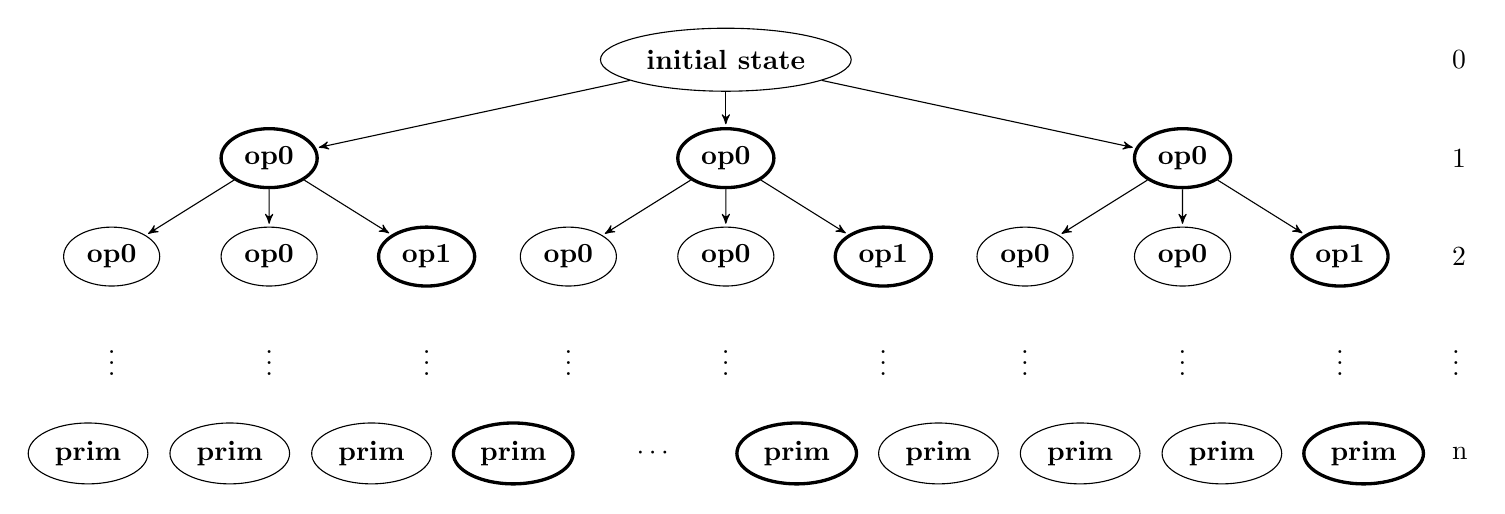
\begin{tikzpicture}[->,>=stealth',shorten >=1pt,auto,node distance=3cm,
                    	main node/.style={ellipse,draw},
		no edge from this parent/.style={
       			 every child/.append style={
        			edge from parent/.style={draw=none}}},
		no outline/.style={
        			every child/.append style={
       			edge from parent/.style={draw=none}}},
	          	level 1/.style = {sibling distance=5.8cm},
    		level 2/.style = {sibling distance=2cm},
    		level 4/.style = {sibling distance=1.8cm},
    		level distance = 1.25cm]
			
\node (Root) [ellipse,draw, minimum width=3cm,minimum  height=.8cm] {\textbf{initial state}}
    child{ node [main node,very thick] {\textbf{op0}} 
            child{ node [main node] {\textbf{op0}} [no edge from this parent]
	 	child{ node {$\vdots$}}}
            child{ node [main node] {\textbf{op0}} [no edge from this parent]
	 	child{ node {$\vdots$}}}
            child{ node [main node,very thick] {\textbf{op1}} [no edge from this parent]
	 	child{ node {$\vdots$}}}           
    }
    child{ node [main node,very thick] {\textbf{op0}}
            child{ node [main node] {\textbf{op0}} [no edge from this parent]
	 	child{ node {$\vdots$}}}
            child{ node [main node] {\textbf{op0}} [no edge from this parent]
	 	child{ node {$\vdots$}
			child{ node [main node] {\textbf{prim}}}
			child{ node [main node] {\textbf{prim}}}
			child{ node [main node] {\textbf{prim}}}
			child{ node [main node,very thick] {\textbf{prim}}}
				child{ node {$\cdots$}[no outline]}
			child{ node [main node,very thick] {\textbf{prim}}}
			child{ node [main node] {\textbf{prim}}}
			child{ node [main node] {\textbf{prim}}}
			child{ node [main node] {\textbf{prim}}}
			child{ node (Root-1-1-1-1) [main node,very thick] {\textbf{prim}}}
		}
	 }
            child{ node [main node,very thick] {\textbf{op1}} [no edge from this parent]
	 	child{ node {$\vdots$}}}  
    }
    child{ node (Root-1) [main node,very thick] {\textbf{op0}}
            child{ node [main node] {\textbf{op0}} [no edge from this parent]
	 	child{ node {$\vdots$}}}
            child{ node [main node] {\textbf{op0}} [no edge from this parent]
	 	child{ node {$\vdots$}}}
            child{ node (Root-1-1) [main node,very thick] {\textbf{op1}} [no edge from this parent]
	 	child{ node (Root-1-1-1) {$\vdots$}}}  
    }
;
 \begin{scope}[every node/.style={right}]
   \xdef\level{Root}  % Initial top level
   \def\rightmostnode{Root-1-1-1-1}   % Name of the node with greater x coordinate
   \foreach \text in {0, 1, 2, $\vdots$ , n}
   {
      \path (\level -|\rightmostnode) ++(5mm,0) node{} ++(5mm,0) node {\text};
      \xdef\level{\level-1}
   }
 \end{scope}

\end{tikzpicture}
} % end for resize

 \caption{Planning tree with $k=3$, where op$x$ indicates an operator at abstraction level $x$ and prim represents a primitive action. There are $n$ levels in the tree.}
 \label{hpn tree}
\end{wrapfigure}

\section{Problem Specification}

\section{Domain Description}

In this section we will discuss our application of BHPN to the UAV domain. Each component described in Section~\ref{bhpn description} will be given in detail as it applies to our UAV mission environment. We will discuss the fluents used to describe the environment as well as the operators used to plan in this environment. The regression functions used in the regression search will be outlined, as well as our realistic observation model.

\subsection{Operators} \label{domain operators}

Below is the list of operators for our UAV domain. They consist of the UAV actions pertaining to our particular mission objectives. In our mission environment there are partially observable ground troops, target, and threats. Our initial belief about their locations is limited, thus we need an Observe operator which gives us (noisy) location information. The UAV itself is fully observable with deterministic actions in our example. Therefore, the Fly operator does not have a probability associated with it, and neither does the uavLoc() fluent. In the operators below, an object can be a target, a threat, or ground troops. There is only one UAV. The fluents are described below, then the generators, and finally the operators. Each operator has a short description along with it.
\\\
\begin{center}
\textbf{Fluents} 
\end{center}
clearPath(path, $p$) : path is free of threats with at least probability $p$ \\
uavLoc(UAV) = loc : the UAV is located at loc \\
uavState(UAV) = state for state $\in$ \{none, relay, prosecute, jamming\} \\
objLoc(obj, $p$) : The obj's location is known with at least probability $p$ \\
objState(obj) = state for state $\in$ \{none, prosecuted, jammed, tracked\} \\
objType(obj) = type for type $\in$ \{threat, target, gt\} \\
surveyed(region) : the given region has been surveyed within the last 10 seconds  \\
havePermission(UAV, threat) : The UAV has permission to prosecute the given threat \\
suppliesDelivered() : The UAV has successfully delivered supplies to the ground troops \\
greaterThan(obj, $p$) : The probability of obj being in its most likely location is greater than \\
\indent  $p$ \\

\begin{center}
\textbf{Generators} 
\end{center}
path = genFastestPath(start, dest) : path is the fastest path from start to dest \\
path = genSurveyPath(start, dest) : path covers the entire rectangular region between start \\
\indent and dest\\
loc = genLikelyLoc(obj) : the obj is most likely located at loc \\
loc = genRelayLoc(gtLoc) : a location in which the UAV has a LOS to the ground troops \\
\indent as well as the control tower \\
(start, dest, loc) = genRegionEndPoints(region) : given a region, determine where the UAV \\
\indent must start and end its surveying given its current location\\

\begin{center}
\textbf{Operators}
\end{center}
\textbf{Fly}(UAV, start, dest, path) \\
\textbf{Preconditions:} \\
\indent 0: uavLoc(UAV) = start \\
\indent 1: clearPath(path, $p_{fly}$) \\
\textbf{Generators:} \\
\indent path = genFastestPath(start, dest) \\
\textbf{Effect:} uavLoc(UAV) = dest \\
The Fly operator moves the UAV from start to dest along the generated path. First, the UAV verifies that the path is clear and then it verifies that the UAV is in the correct starting location. As it flies it is also observing its surroundings and updating the survey times in the cells it passes through.
\\\
\\\
\textbf{Observe}(UAV, object, loc, $p$): \\
\textbf{Preconditions:} \\
\indent 0: objLoc(object, $regress(p)$) \\
\indent 1: greaterThan(object, $p_{observe}$) = True \\
\indent 2: uavLoc(UAV) = loc \\
\textbf{Generators:} \\
\indent loc = genLikelyLoc(object) \\
\textbf{Effect:} objLoc(object, $p$) \\
The Observe operator allows the UAV to increase its knowledge about an object's location to $p$. The first precondition is that the object's location is known with at least $regress(p)$. The Observe action can only be taken if the object's initial probability ($regress(p)$) is greater than some threshold value, $p_{observe}$. If it is not, then the UAV must get the object's location from the ground troops (see below). Lastly, the UAV must be located in the most likely location of the object.
\\\
\\\
\textbf{GetInfoFromGT}(UAV, gt, object, $p$) \\
\textbf{Preconditions:} \\
\indent 0:  greaterThan(object, $p_{observe}$) = False\\
\indent 1: objLoc(gt, $p_{gtLoc}$) \\
\indent 2: objLoc(object, $regress(p)$)\\
\indent 3: uavLoc(UAV) = loc \\
\textbf{Generators:} \\
\indent loc = genLikelyLoc(gt) \\
\textbf{Effect:} objLoc(object, $p$) \\
GetInfoFromGroundTroops allows a UAV to gather information regarding an object's location through communication with the ground troops. The preconditions are the same as the Observe action with two exceptions. First, the UAV must know the ground troops location with at least $p_{gtLoc}$, and second the object's initial belief must be below $p_{observe}$ (as opposed to the Observe action where is had to be above $p_{observe}$).
\\\
\\\
\textbf{Survey}(UAV, region, start, dest, path) \\
\textbf{Preconditions:} \\
\indent 0: clearPath(path, $p_{fly}$) \\
\indent 1: uavLoc(UAV) = start \\
\textbf{Generators:} \\
\indent (start, end) = genRegionEndpoints(region) \\
\indent path = genSurveyPath(start, end) \\
\textbf{Effect:} surveyed(region) \\
Survey allows the UAV to gather information about a specific region. A zig-zag path is generated through the region such that every cell is within the UAV's visibility radius at one point. First, the UAV verifies that this path is clear and then it checks that it is in the correct starting location.
\\\
\\\
\textbf{Track}(UAV, object, loc) \\
\textbf{Preconditions:} \\
\indent 0: objType(object) $\neq$ threat\\
\indent 1: objLoc(obj, $p_{track}$) \\
\indent 2: uavLoc(UAV) = loc \\
\textbf{Generators:} \\
\indent loc = genLikelyLoc(object) \\
\textbf{Effect:} objState(object) = tracked \\
The Track operator enables a UAV to track an object (if it is not a threat). First, the UAV verifies that the object is not a threat. Second, it must know the object's location with at least $p_{track}$. Finally, it ensures that the UAV is located in the most likely location of the object.
\\\
\\\
\textbf{ClearPath}(UAV, path) \\
\textbf{Preconditions:} \\
\indent 0: threatState(threat) = prosecuted for threat $\in$ threatsInPath\\
\textbf{Generators:} \\
\indent threatsInPath = genThreatsInPath(path) \\
\textbf{Effect:} clearPath(path) \\
The ClearPath operator is what changes a path from not being clear to being clear. First, it generates a list of all threats in the path. Then it makes a list of preconditions which state that each threat in the path must be prosecuted before the path can be cleared.
\\\
\\\
\textbf{Prosecute}(UAV, threat) \\
\textbf{Preconditions:} \\
\indent 0: havePermission(UAV, threat) \\
\indent 1: objLoc(threat, $p_{prosecute}$) \\
\indent 2: uavLoc(UAV) = loc \\
\textbf{Generators:} \\
\indent loc = genLikelyLoc(threat) \\
\textbf{Effect:} objState(threat) = prosecuted \\
This operator allows a UAV to prosecute a threat. First the UAV checks that it has permission from the human operator. Then it ensures that it knows the threats location with at least $p_{prosecute}$. Then it moves the UAV to the threat's most likely position.
\\\
\\\
\textbf{Jam}(UAV, threat) \\
\textbf{Preconditions:} \\
\indent 0: havePermission(UAV, threat) \\
\indent 1: objLoc(threat, $p_{jam})$ \\
\indent 2: uavLoc(UAV) = loc \\
\textbf{Generators:} \\
\indent loc = genLikelyLoc(threat) \\
\textbf{Effect:} objState(threat) = prosecuted \\
The Jam operator causes the UAV to jam a threat's electronic attacking capabilities. First, the UAV must be given permission to perform the jamming action. Then it verifies that it knows the threat's location with at least $p_{jam}$, and finally it moves the UAV to the threat's most likely location.
\\\
\\\
\textbf{DeliverSupplies}(UAV, gt) \\
\textbf{Preconditions:} \\
\indent 0: objLoc(gt, $p_{deliver}$) \\
\indent 1: uavLoc(UAV) = loc \\
\textbf{Generators:} \\
\indent loc = genLikelyLoc(gt) \\
\textbf{Effect:} suppliesDelivered() \\
Sometimes it may be necessary for a UAV to deliver supplies to ground troops. In order to perform this action, a UAV must know the ground troop's location with at least $p_{deliver}$. Then the UAV must most to the ground troop's most likely position in order to deliver the supplies.
\\\
\\\
\textbf{Relay}(UAV, gt) \\
\textbf{Preconditions:} \\ 
\indent 0: objLoc(gt, $p_{relay})$ \\
\indent 1: uavLoc(UAV) = relayLoc \\
\textbf{Generators:} \\
\indent gtLoc = genLikelyLoc(gt) \\
\indent relayLoc = genRelayLoc(gtLoc) \\
\textbf{Effect:} uavState(UAV) = relay \\
When communication is lost between the ground troops and the control tower, the UAV may be needed to act as a relay between the two. In order to do this the UAV must know the location of the ground troops with at least $p_{relay}$, and then must be situated at the relay location where it has a LOS between both the UAV and the ground troops.

\subsection{Regression Functions}

Regression functions are used to calculate necessary precondition probabilities based on required effect probabilities. For example, if a UAV needs to know the location of a target with 0.9 certainty, how certain must is \textit{currently} be about the target's position? These functions depend on the UAV's sensor capabilities. If the sensor has little noise, then the UAV can be confident that it will achieve the goal of 0.9 certainty. However, if the UAV has a very noisy sensor, it will need a higher certainty as a precondition to execute the observe operator. The regression functions are best-case, and are computed under the assumption that we are directly overhead the target we are observing and we do not receive a false positive. Below is the regress function where $p_{cp}$ is the probability of a correct positive, and $p_{fn}$ is the probability of a false negative. It is derived from the UAV's observation model, which we will discuss in Section \ref{uav domain observation}.

\begin{equation}
\text{regress}(p) = \frac{p_{cp}p}{(1-p)p_{fp} + p_{cp}p}
\end{equation}

\subsection{Observation Model} \label{uav domain observation}

In UAV missions, observations are acquired through UAV camera data using object recognition algorithms. However, our research focuses on planning and not object recognition. In our simulated environment camera data is modeled as a process with Gaussian noise and no data association errors. In other words, the observations consist of the object being identified with no error, and the location of that object with Gaussian noise. There is also a chance of either incorrectly missing an object which is visible (false negative), or seeing an object when it is not visible (false positive). There is a visibility radius around the UAV so that if an object is detected, it must be within this radius. 

The observations, $\mathbf{z}_{k}$, are functions of the underlying object states, $o_{k}$. The range of the UAV's camera visibility is characterized by a radius, $r$, and the state of the UAV is $\mathbf{x}_{k}$. We designate R($\mathbf{x}_{k}$) to be the set of states within $r$ of the UAV at time step \textit{k}. 

\begin{equation}
\text{R}(\mathbf{x}_{k}) := \{s\text{ } | \text{ } ||\mathbf{x}_{k} -  s|| < r\} \text{ where } s \in \mathbb{R}^{2}
\end{equation}

\begin{equation}
\mathbf{z}_{k} \in \{ (x_{k},y_{k})\} \text{   where   }  (x_{k},y_{k}) \in \text{R}(\mathbf{x}_{k})
\end{equation}

$P(\mathbf{O}_{k})$ is the probability distribution of an object's location over all possible states. 
For example, if an object's state is known with absolute certainty, $P(\mathbf{O}_{k} = o_{k}) = 1$. For the remainder of this section the $k$ subscript is dropped for ease of reading.

The following formalization of the observation model is based on Dille~\cite{dille2013search}. If an object is in R($\mathbf{x}$), there are three possible observations: the object is detected and the observation is correct, the object is detected but the observation is incorrect, or the object is not detected. We will refer to an incorrect object position as $o_{incorr}$. If the object is not in R($\mathbf{x}$), then there is a chance of a false positive occurring. The table below outlines all of these possibilities and the probabilities associated with each of them.

\begin{center}
\begin{tabular}{ | l | l | l |}
\hline
                                                                               & $o \in$ R($\mathbf{x}$)                                                                                & $o \notin$ R($\mathbf{x}$) \\ \hline
$\mathbf{z} = \emptyset$                                    & $P(\mathbf{z}=\emptyset|o) = 1-p_{cp}$                                                    & $P(\mathbf{z}=\emptyset| o) =1-p_{fp}$\\ \hline
$\mathbf{z} \in \text{R}(\mathbf{x})$                 &  \shortstack[l] {$P(\mathbf{z} = o|o) =p_{cp}[\mathcal{N}(\mathbf{o}|\mathbf{x},\sigma^{2})] $ \\
				                                         $P(\mathbf{z} = o_{incorr}|o) =p_{cp}[1-\mathcal{N}(o|\mathbf{x},\sigma^{2})] $    }                
																		         & $P(\mathbf{z}=o_{incorr}|o)=p_{fp}$\\ \hline
\end{tabular}
\end{center} 

The variables $p_{cp}$ and $p_{fp}$ are the probabilities of a correct positive and a false positive, respectively. Within the UAV's visibility radius, observations are Gaussian. $\sigma$ is the variance which characterizes the performance of the target recognition algorithm. The greater it is, the better the UAV can detect objects that are far away, and vice versa. During plan execution, the observations and the observation model above are used to update object belief states through Bayes filtering. 

\section{Complexity Analysis}
\subsection{BHPN Complexity}

As mentioned in Section~/ref{bhpn algorithm}, hierarchical planning is efficient because it develops multiple plans of length $k$, which are shorter in length than the final plan, $l$, they are contributing to. The length of the final plan is the number of leaf nodes in the planning tree. Flat planning is the method of planning without the use of abstraction. In flat planning there is no recursion and all preconditions are considered simultaneously. This problem is much more constrained than the hierarchical problem, and the solution complexity grows exponentially with the overall plan length.

The complexity of hierarchical planning depends on the planning tree depth, $n$, the number of operators added per subgoal, $k$, and the total number of possible operators, $b$. Assume the tree is regular, or all nodes have $k$ children. Each level, $i$, of the tree represents an ordered plan of length $k^{i}$. Level $n$ represents an executable plan of length $l = k^{n}$. The work done in expanding each node is $b^{k}$. Therefore, to calculate the overall complexity of the planning tree we must sum up the work for each level: $ \sum_{i=1}^{n} k^{i}b^{k}$, which gives  $O(lb^{k})$ or $O(b^{k})$. If flat planning had been used, then the complexity would be $O(b^{l})$ as opposed to $O(b^{k})$. This shows the savings generated by hierarchical planning, since $k=l^{1/n} << l$. 

This analysis assumes that all plans are refineable and no backtracking is necessary, all actions are permanent and there is no replanning, and all plans serialize or no subgoals interact. There are two instances where these assumptions do not hold. First, in a dynamic world, not all actions are permanent. For example, if a target is dynamic, then it may be necessary to localize it several times throughout a mission to ensure that we still know where it is. In this case actions are not permanent. Second, subgoals may interact if the action of one undoes a precondition of the other. 

This analysis only accounts for the task planning component of the overall BHPN algorithm. The motion planning complexity is dependent on the motion planning algorithm in place. For our simulation we implemented A* for UAV motion planning. To evaluate a \textit{combined} task and motion planner is difficult due to the heavy reliance on current belief state and mission objectives. Some missions may prove to be very difficult in a motion planning sense due to the number of threats in the world. Other missions might be very easy to execute in a motion planning sense, but the goal contains five fluents, therefore complicating the task planning. 

\subsection{Suboptimality and Reachability}

\section{Single-Agent Planning}

\subsection{Mission Scenarios}

Below are examples of mission scenarios which we simulated in Gazebo using ROS (robotic operating system). \\

\noindent
\textbf{objState(target1) = tracked} \\
The UAV needs to track target1. First it verifies that target1 is not a threat. Then, it needs to increase its belief about the location of target1 to at least $p_{track}$. First, it attempts to directly observe target1 (because the initial belief is above $p_{observe}$) but then it doesn't see it there, and the belief drops below $p_{observe}$. So it attempts to get information from the ground troops. The ground troops give the correct location and the UAV goes back to directly observing target1's most likely location (given the information from the ground troops), and is finally able to directly observe the target. Once its belief of target1's location is above $p_{track}$ then the UAV enters track mode, and continues to track the target. \\

\noindent
\textbf{surveyed(region1) = True} \\
To survey region1, first the UAV generates a path which will cover the entire region. Then it begins to move along this path. While flying along this path, it detects a threat in the perimeter of its visibility radius. In order to survey the entire region, the UAV must cover the region currently occupied by the threat. So, the UAV asks permission from the operator to prosecute the threat. Permission is given, the UAV prosecutes the threat, and continues to fly along this path until all of region1 has been surveyed. While flying, the UAV is also gather information about new objects and updating the beliefs of objects which it has already seen. \\

\noindent
\textbf{objState(threat1) = jammed} \\
First, the UAV has to get permission from the human operator to jam the threat. Then, it must know where the threat is with at least probability $p_{jam}$. The current belief is below $p_{observe}$, so the UAV has to get information from the ground troops regarding the threat's location. Once it has this information it confirms by directly observing the threat until the belief is above $p_{jam}$. Finally the UAV performs the electronic attack, and changes its state such that uavState(UAV) = jamming and objState(threat1) = jammed. \\

\noindent
\textbf{suppliesDelivered() = True and uavState(UAV) = relay} \\
The UAV is tasked with delivering supplies to the ground troops, then acting as a relay between the ground troops and control tower. Assuming the UAV has supplies with it, the UAV must verify the location of the ground troops and increase its belief to above $p_{deliver}$. Once this is done, it can drop the supplies down to the ground troops. Then, using its current location (above the ground troops) and the control tower location, it determines the best (least threatening) location where it can achieve a LOS between the ground troops and control tower, flies there and acts as a relay. \\

\subsection{Simulation Results}

To display the effectiveness of the simulated single-agent mission planner we have developed, Figure~\ref{tree-1} gives a hierarchical plan decomposition. The mission objective is to localize a specific target. The UAV has very little initial belief about the location of the target, but a high certainty of where the ally ground troops are located. It gets target location information from the ground troops, then confirms the target location with direct sensing. The green nodes in the figure represent the primitive actions.

\begin{figure}
 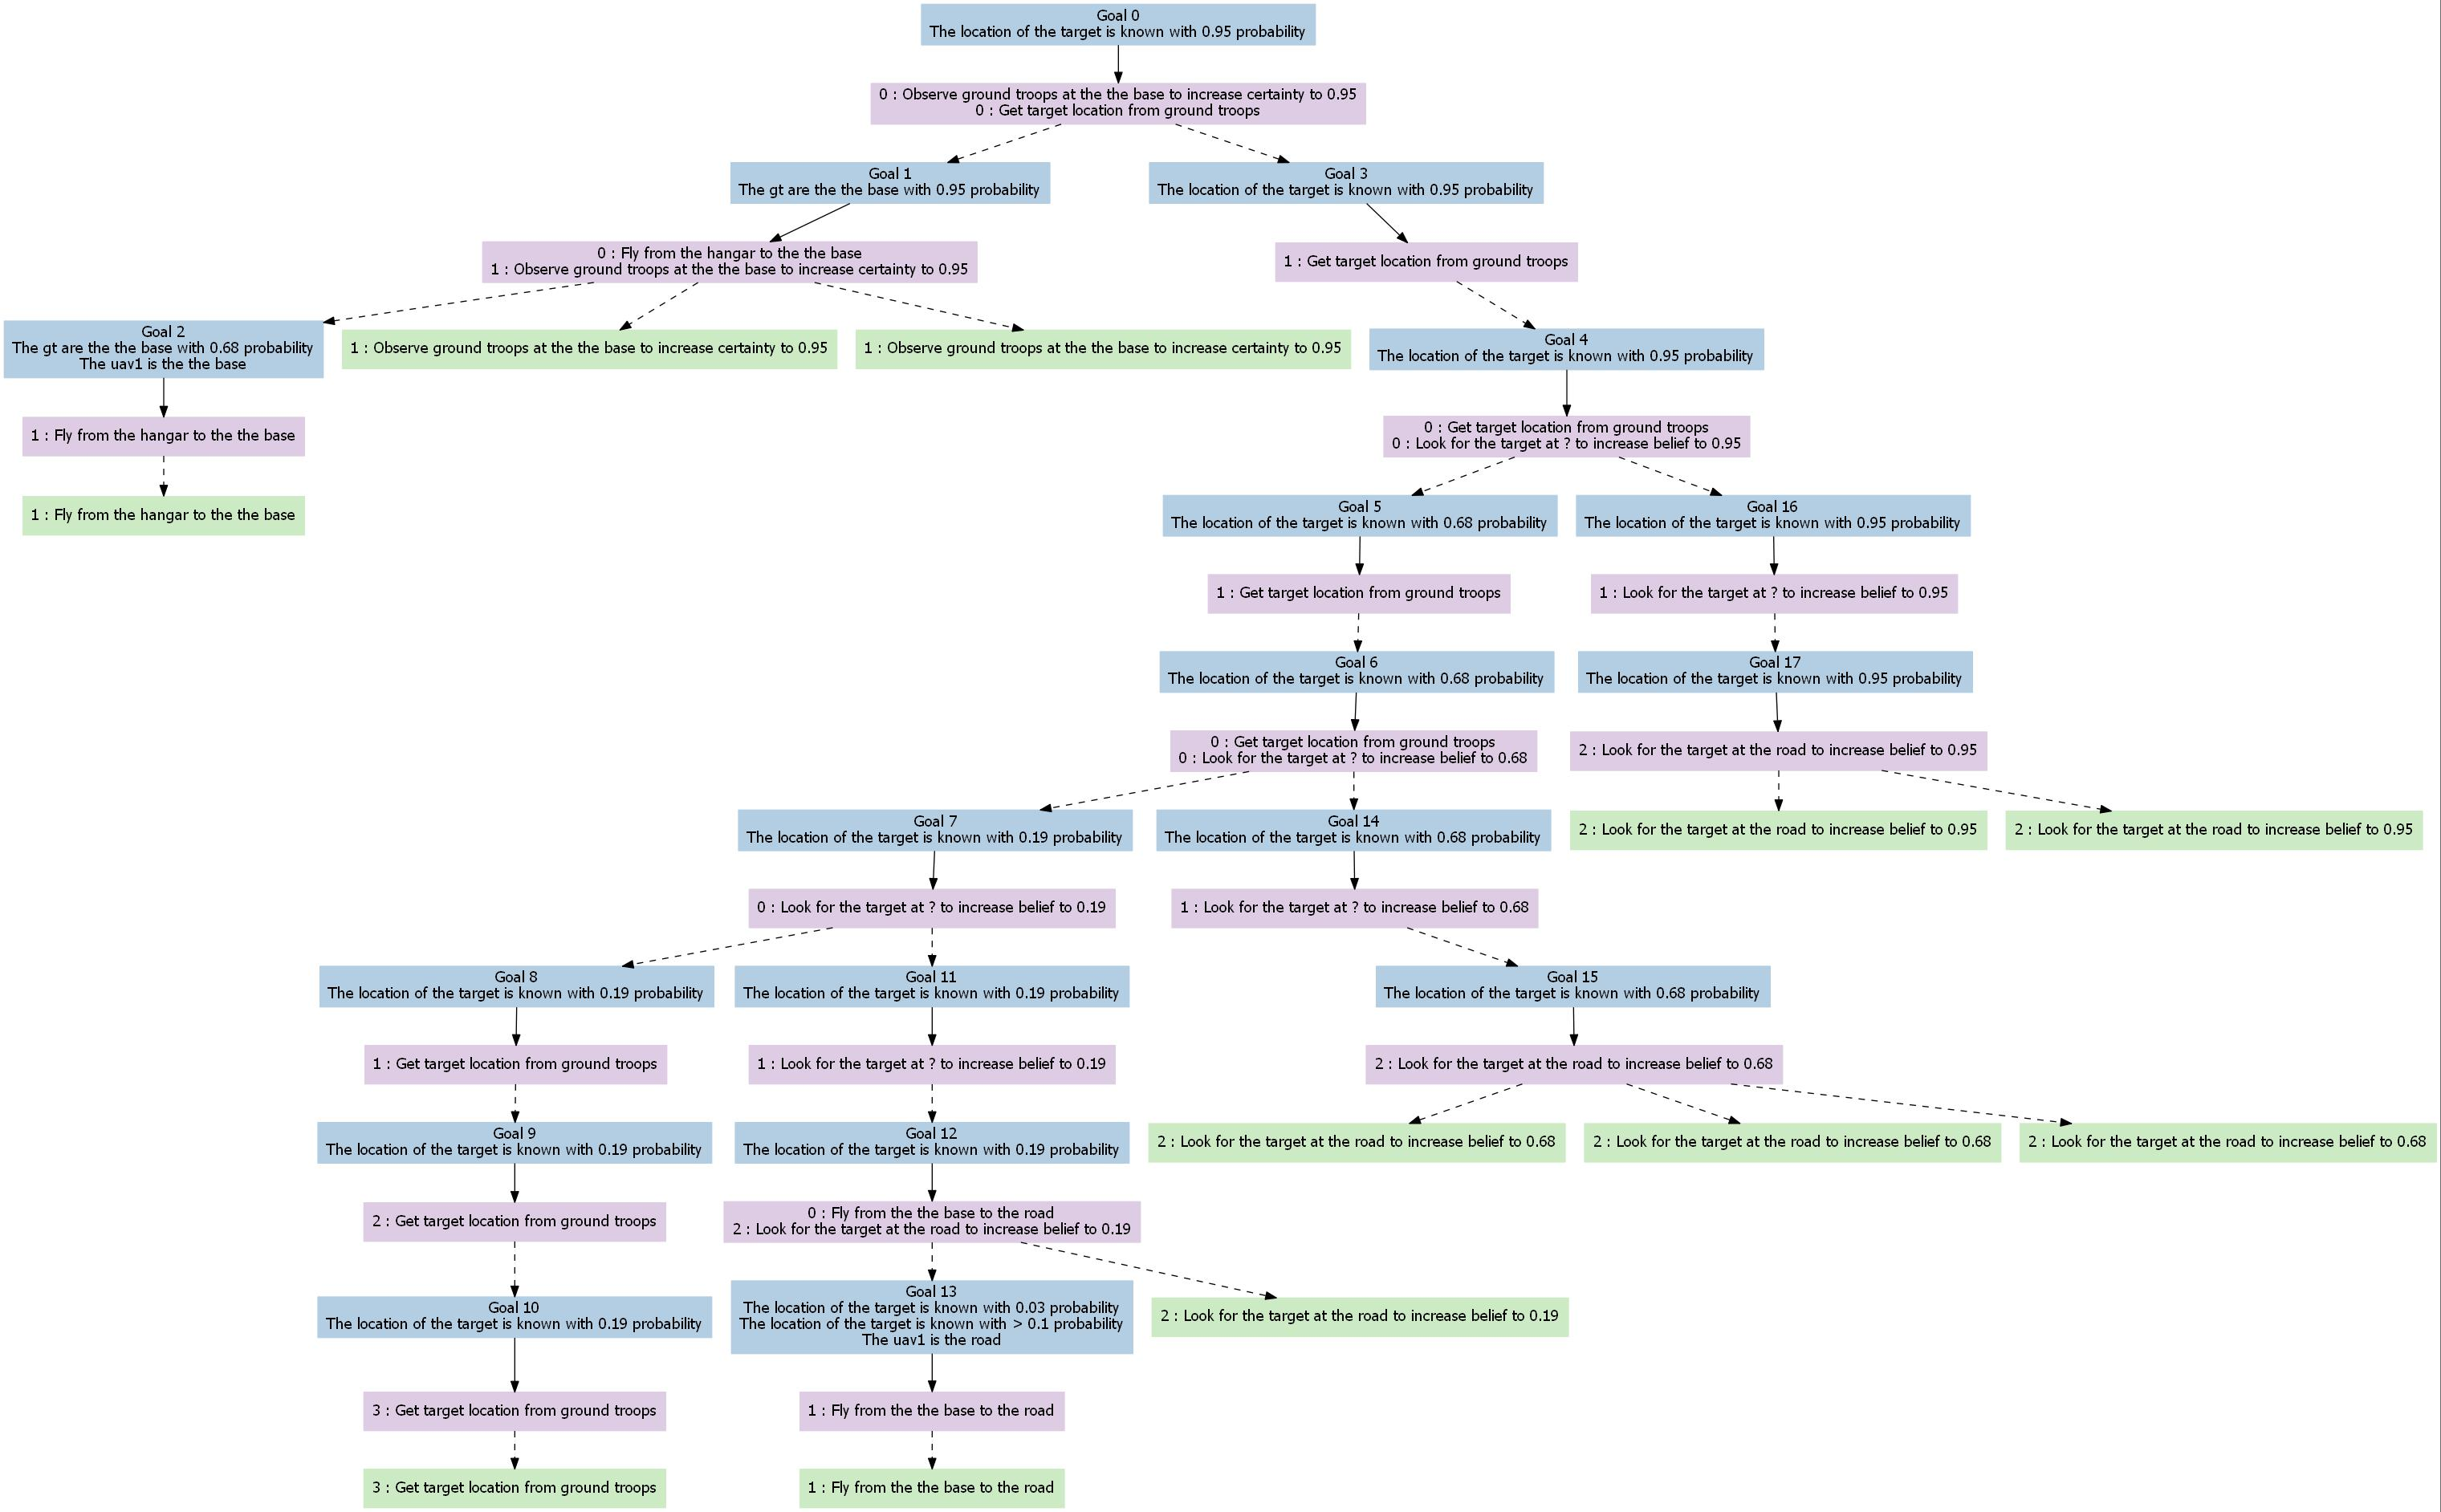
\includegraphics[width=18cm]{example-tree1}
 \caption{This is the planning tree constructed while accomplishing the overall goal of knowing the target location with 0.95 certainty (Goal 0). The blue nodes represent goals and subgoals (or pre-images), the pink nodes represent plans, and the green nodes represent primitive actions being executed. The numbers before each operator in the plan nodes are the respective operator abstraction levels.}
 \label{tree-1}
\end{figure}

\section{Multi-Agent Planning}

In this mission environment, multiple UAVs are used to achieve different objectives. The UAVs are heterogeneous, meaning that they all have different abilities. For example, one UAV may be the only one with the ability to prosecute, while another is the only one with the ability to act as a relay. In this environment, all UAVs are knowledgeable about their own and each other's abilities. All operators will remain the same as they are for single-agent task planning, except for one key difference. The first precondition of all operators will be:
\begin{center}
\textbf{isAvailableUAV(`UAV')}
\end{center}

When this precondition is being evaluated, a genUAV() generator will be called. In single-agent task planning this generator would always bind the acting UAV to the `UAV' argument. However, in multi-agent task planning, this generator will be more complicated. It will have access to all UAV's abilities, as well as the UAV attempting to execute this operator, and it will bind a UAV that is able to complete this task. It will always check the UAV making the call first, to see if it is capable of performing this action. If it is not, then it will ask other UAVs with this capability is they are available to help. If none of them are, then it will bind `None' to the `UAV' arg, and the isAvailableUAV(`UAV') fluent will evaluate to be False, and planning will fail.

In this environment, each UAV has its own goal that it is trying to satisfy. Planning is decentralized. Since planning is decentralized, in order for a UAV to receive help, there needs to be a method of ranking the importance of one's own current primitive or overall goal against the importance of another agent's objective (the one who is asking for help). In our implementation we achieve this by ranking the importance of each operator. When a UAV is being asked to help another, it compares the operator it is currently executing to the one it is being requested to perform, and chooses which is more important.

\subsection{Mission Scenario}

Below are two examples of multi-agent mission scenarios:\\

\noindent
UAV1 is given the goal of tracking Target1. However, there are threats in the path to Target1 and UAV1 does not have the ability to prosecute threats (which is the only way to clear the path). UAV2 is given the goal of surveying Region1. UAV2 has the ability to prosecute threats. Since the survey action isn't as critical as prosecuting threats, UAV2 is available to help UAV1.  UAV1 asks for help (through the isAvailableUAV() precondition). When it is confirmed that UAV1 will be receiving help, it then tries to satisfy the necessary prosecute preconditions. UAV1 gets permission from the human operator to prosecute and localizes the threat. Finally, UAV2 comes in to help and prosecutes the threat while UAV1 loiters nearby. Afterwards UAV2 continues to survey Region1 (as it had previously been doing). UAV1 flies the newly cleared path towards Target1, localizes it, and begins tracking it.\\

\noindent
UAV1 is trying to deliver supplies to the ground troops, but its sensing capabilities are not adequate enough to localize the ground troops. UAV2's current goal is to act as a relay between the ground troops and the control tower. First, UAV1 asks UAV2 for help and receives it. UAV2 aborts its current goal, localizes the ground troops, then returns to acting as a relay. UAV1 is now able to deliver the supplies.

\subsection{Simulation Results}

\section{Evaluation}
\subsection{POMDP Comparison}

Solving a POMDP optimally can be done for some small finite horizon problems with a small state space, using the optimal value iteration algorithm. This value function can be represented by a set of $|S|$-dimensional hyperplanes, $\Gamma_{t}$. They describe a value function over the belief space for a specific action. The best value is then calculated based on these value functions. The complexity of this algorithm is $O(|A||Z||S|^{2}|\Gamma_{t-1}|^{|Z|})$, where $A$ is the size of the action space, $Z$ is the size of the observation space, and $S$ is the size of the state space.

Standard online planning algorithms require building a belief tree of depth D. Evaluating a tree of all reachable beliefs to depth D requires $O((|A||Z|)^{D}|S|^{2})$. This has a few drawbacks: it is exponential in D, and there typically is not enough time at each planning step to fully build and evaluate the entire belief tree. Methods like POMCP and DESPOT efficiently handle these drawbacks.

The complexity of task planning using BHPN is $O(b^{k})$ where $b$ is the number of available operators, and $k$ is the number of actions added each time the HPN tree is refined. Adding certain actions requires calling a path planner. Since the belief space is discretized for planning efforts, the path planner is not required to work in the space of probability distributions, and it assumes that actions are deterministic. Then, as paths are followed during execution, deviations from this assumption are monitored and replanned for. This method is efficient as it does not require planning in belief space, however domain knowledge is required to plan efficiently using BHPN.

\subsection{Multi-Agent Planning Comparison}

\section{Conclusion}

% produces the bibliography section when processed by BibTeX
\bibliography{bibtex_database}
\bibliographystyle{plain}

\end{document}
